%% elementary_tasks.tex
%% Author: Leighton Pritchard
%% Copyright: James Hutton Institute
%% Elementary perceptual tasks, as in Cleveland & McGill (1984)

% ELEMENTARY PERCEPTUAL TASKS
\begin{frame}
  \frametitle{Elementary Perceptual Tasks
  \footnote{\tiny{\href{https://www.jstor.org/stable/2288400}{Cleveland \& McGill (1984) \textit{J. Am. Stat. Ass.}}}}
  }
  \textcolor{hutton_green}{The most basic visual tasks:}
  \begin{center}
    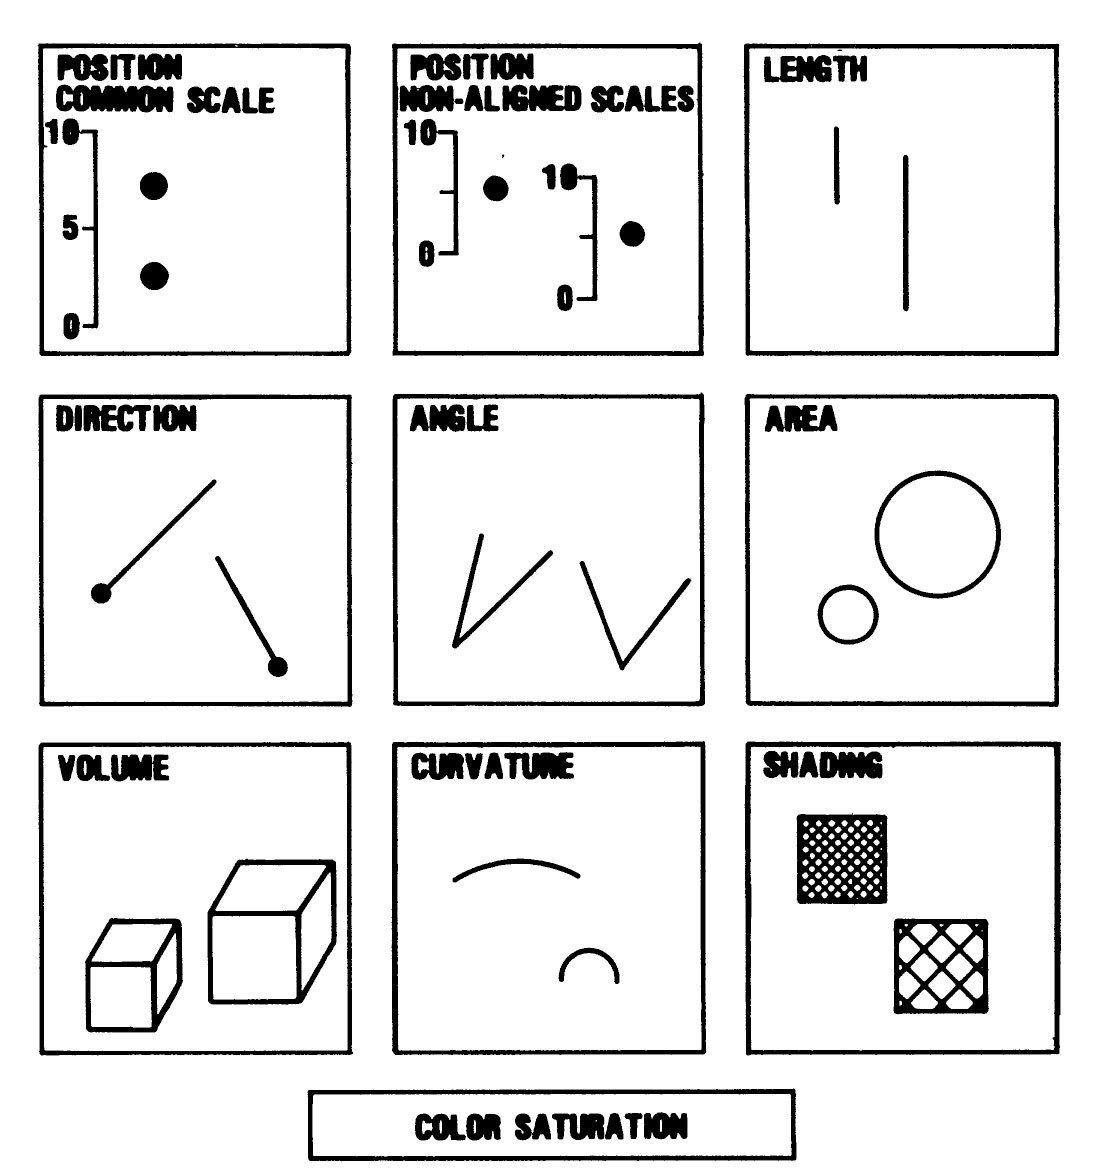
\includegraphics[height=0.7\textheight]{images/elementary_perceptual_tasks}
  \end{center}
\end{frame}

% WHAT IMPLEMENTS THESE?
\begin{frame}
  \frametitle{Implementations
  \footnote{\tiny{\href{http://www.datavizcatalogue.com/}{http://www.datavizcatalogue.com/}}}
  }
  \begin{columns}[T]
    \begin{column}{6cm}  
      \begin{alertblock}{Position: common scale}
        \begin{itemize}
          \item Scatterplot
          \item Bar Chart
        \end{itemize}
      \end{alertblock}
      \begin{block}{Angle}
        \begin{itemize}
          \item Pie Chart
          \item Do(ugh)nut Chart
        \end{itemize}  
      \end{block}
      \begin{alertblock}{Curvature}
        \begin{itemize}
          \item Arc Diagram
          \item Chord Diagram
        \end{itemize}
      \end{alertblock}
      \end{column}
    \begin{column}{4cm}  
      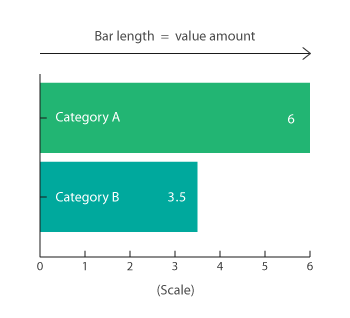
\includegraphics[width=0.65\textwidth]{images/bar_chart} \\
      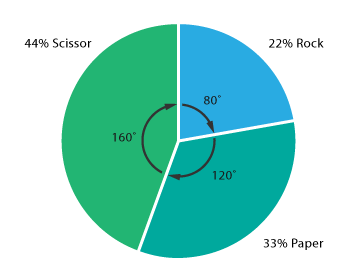
\includegraphics[width=0.65\textwidth]{images/pie_chart} \\
      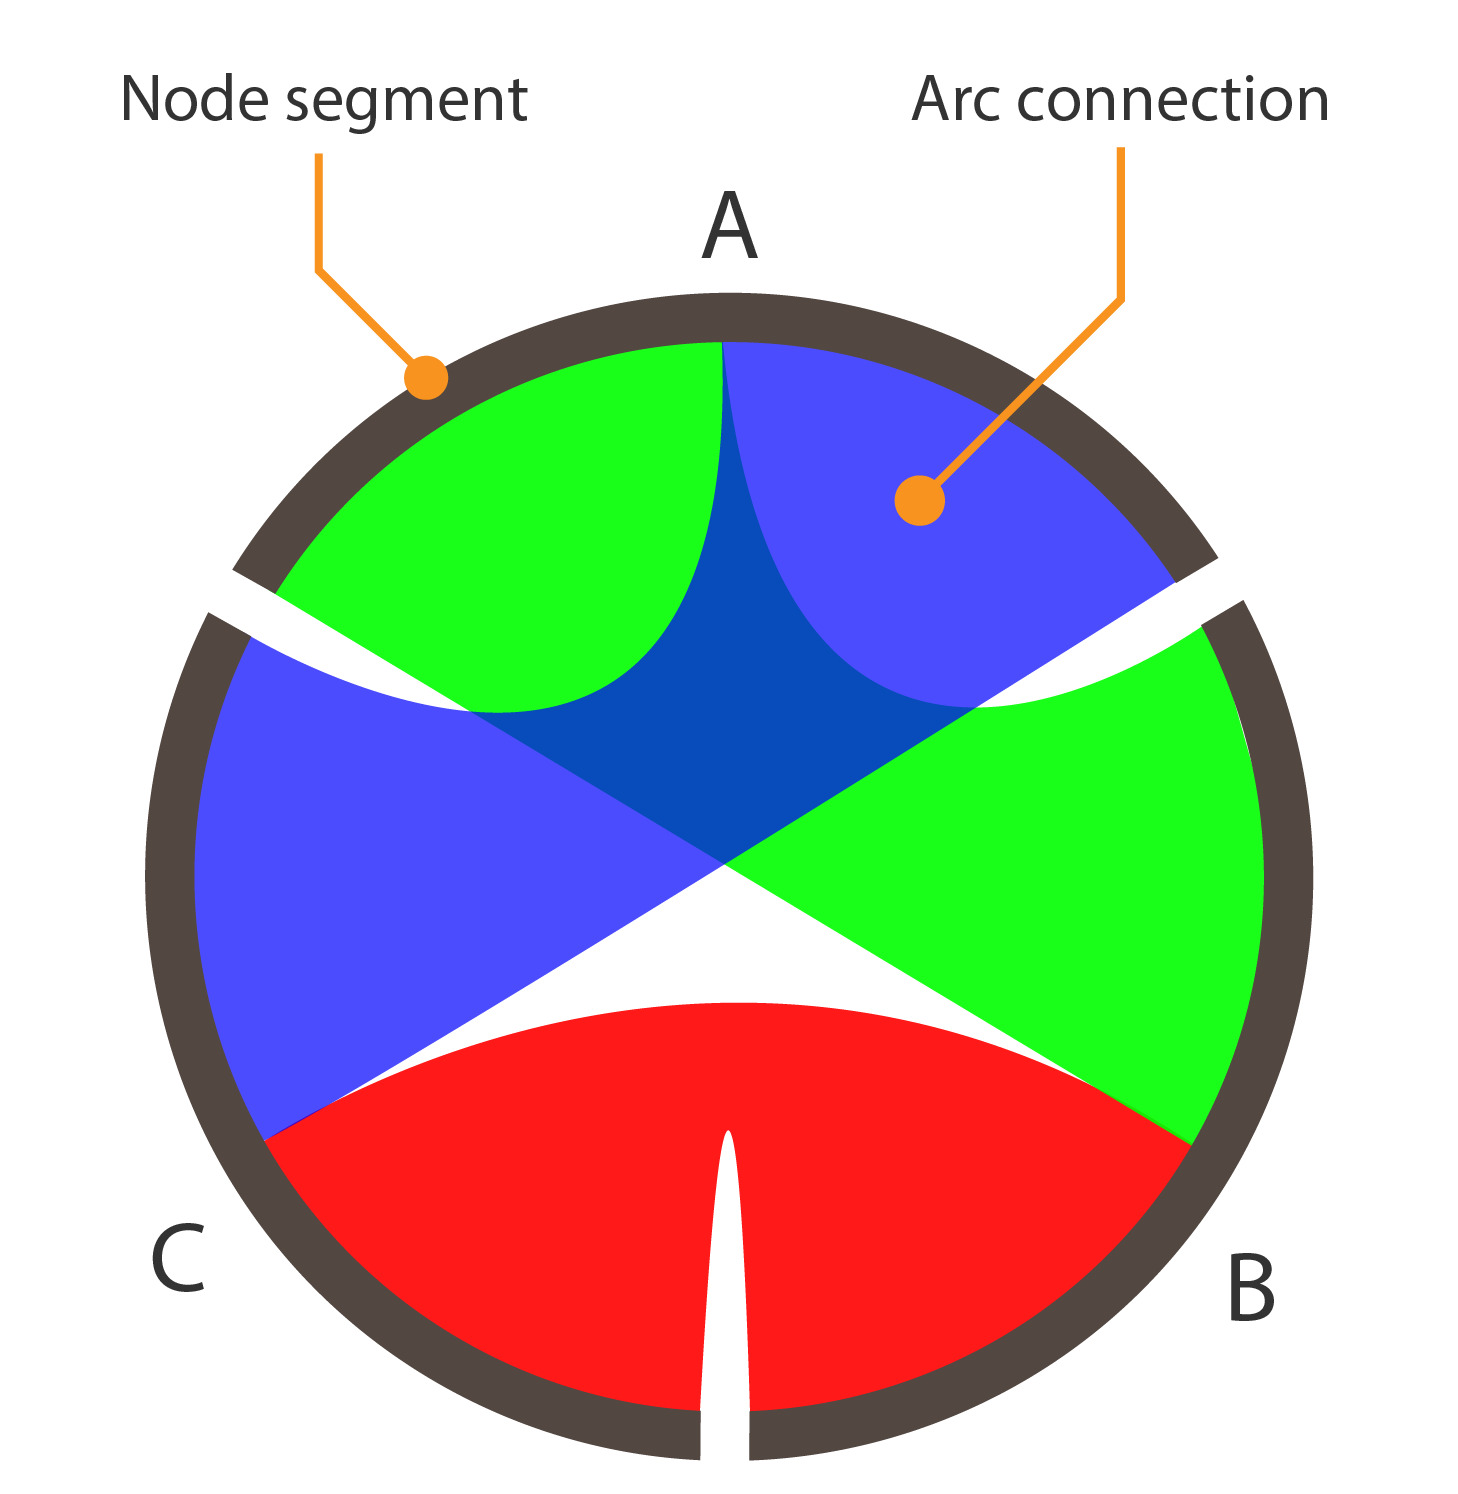
\includegraphics[width=0.65\textwidth]{images/chord_diagram}
    \end{column}
  \end{columns}      
\end{frame}

